\documentclass{article}
\usepackage[utf8]{inputenc}
\usepackage{graphicx}
\usepackage{float}

\author{Hamza Sheikh}

\begin{document}

\subsection{The Importance of Design}

Design is a great initial investment owing to a number of different reasons. Having a design process allows for more efficiency and transparency when actually coming to design the application. It overcomes the risk of having to refer back to the drawing board when actually developing the application, setting in stone the main features and functionality of the application.\\

\subsection{The Unified Modeling Language}

A way in which effective design strategies were carried out was through the implementation of the Unified Modeling Language (UML), a powerful standard for creating specifications of various parts of a software system.\\

\\One example of the UML was our implementation of a use case diagram which outlined the different scenarios in which a user would function the application. See figure~\ref{fig:Use Case Diagram}.\\

\begin{figure}[H]
    \centering
    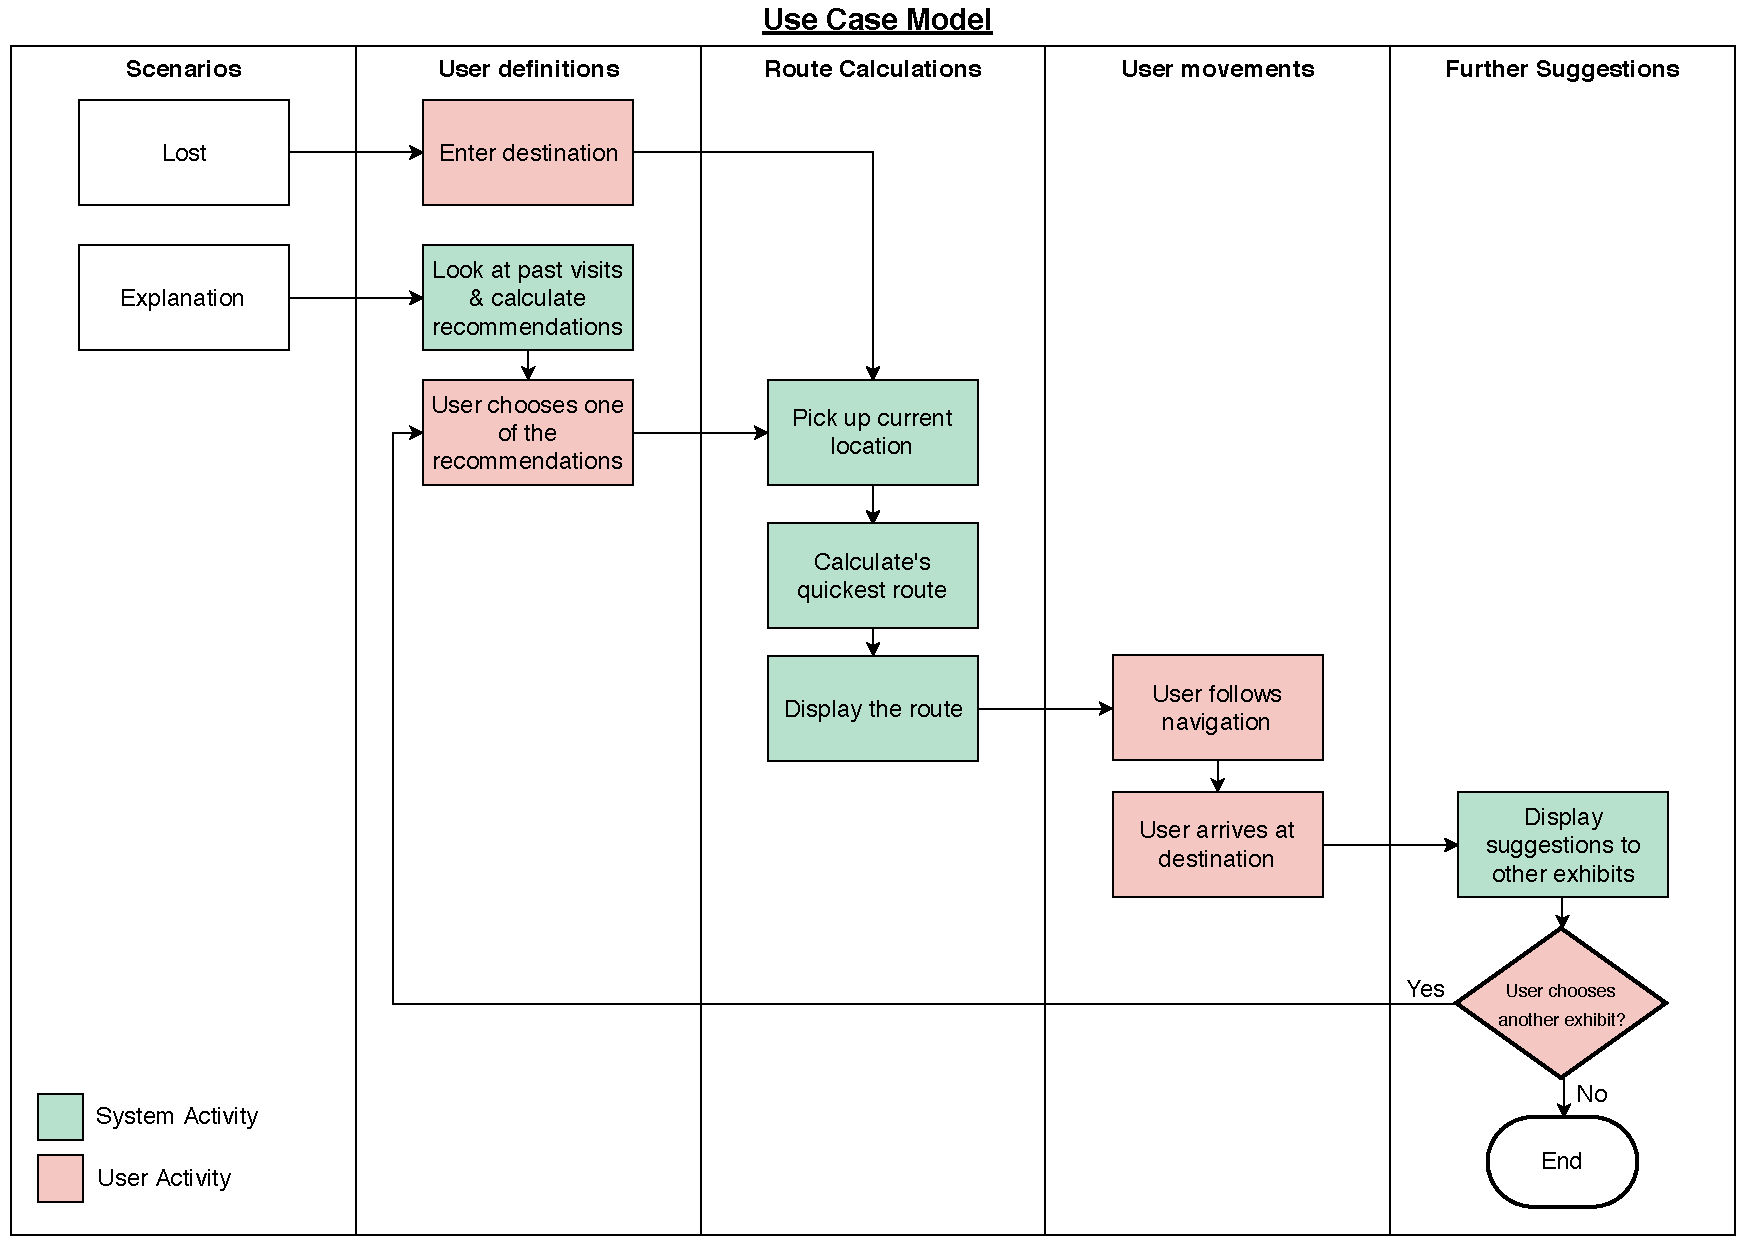
\includegraphics[width=\textwidth]{use_case.pdf}
    \caption{Use Case Diagram}
    \label{fig:Use Case Diagram}
\end{figure}

\\Another way in which UML was implemented to further support and refine the designing phase of the software development was through an activity diagram. (See figure~\ref{fig:Activity Diagram}).

\begin{figure}[H]
    \centering
    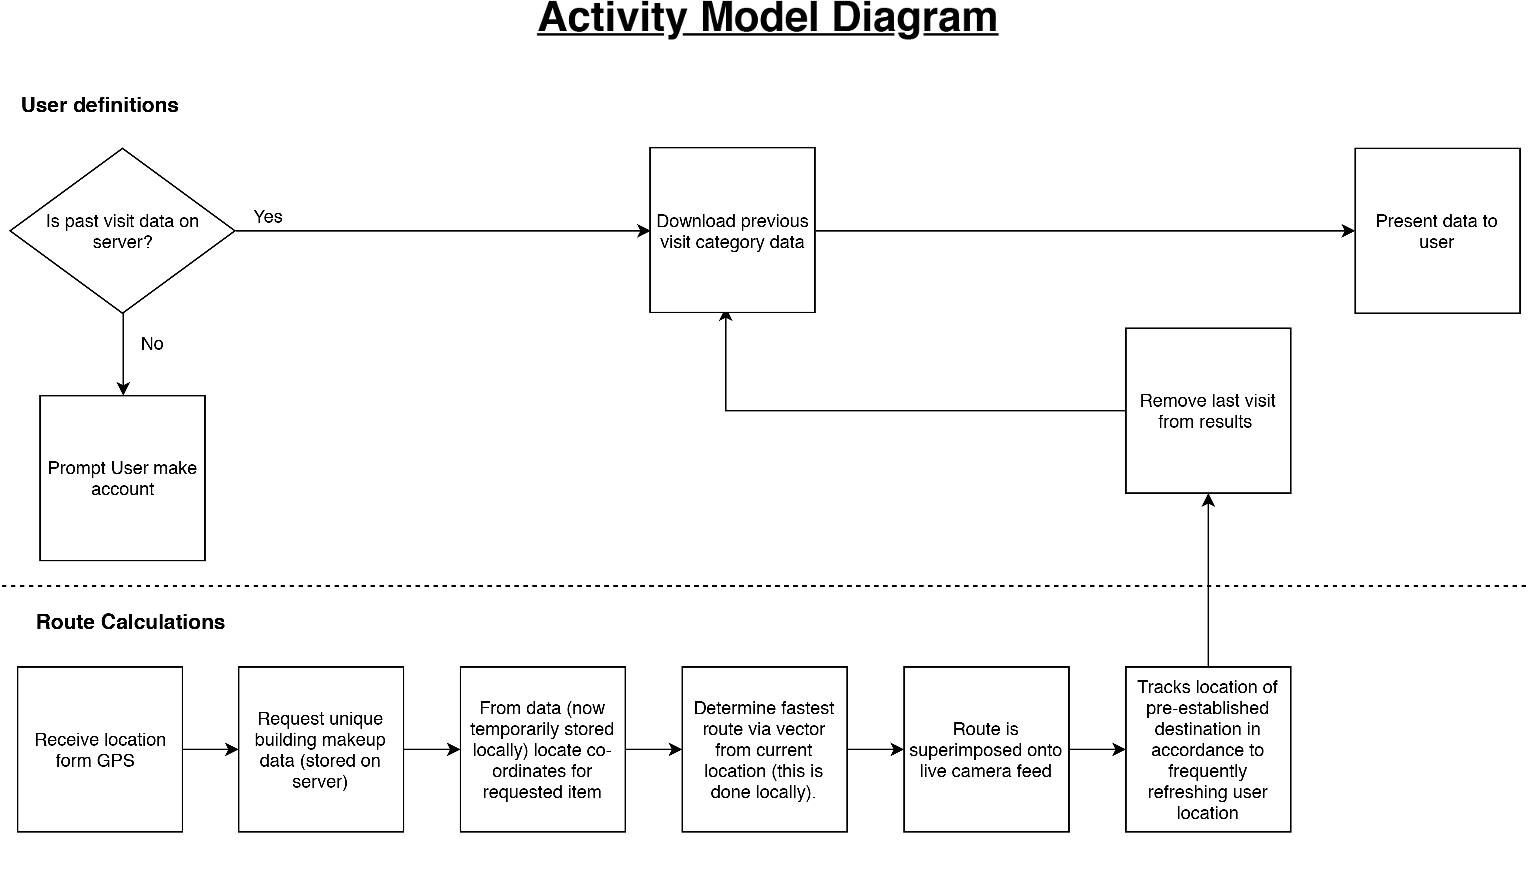
\includegraphics[width=\textwidth]{Activity_Diagram.pdf}
    \caption{Activity Diagram}
    \label{fig:Activity Diagram}
\end{figure}

\\The use case diagram (Figure~\ref{fig:Use Case Diagram}) represents the functional behaviour of the system in terms of goals that can be fulfilled by the system. These goals have been defined in the stakeholder requirements. The activity diagram (Figure~\ref{fig:Activity Diagram}) was designed to model the work flow of the system. One main reason that the activity diagram was essential in the designing phase was that UML included that these diagrams are normally easily comprehensible for both analysts and stakeholders. By producing and creating these models, we were able to have a clear understanding of what the application \textit{has} to do, and enabled us, the developers, to visualise the application for the future.

\subsection{Service Model}

We have to first exclaim that the following cases are born out of one important principle; convenience. The \textbf{'lost'} use case, for example, comes from the fact that the user could be lost for whatever reason. What we would provide through this service would be the quickest and most \textbf{convenient} solution to finding their destination. Whether that be the exit, a cafe or a particular exhibition. Another use case;
\textbf{'exploration'}, would become more convenient with the museum, and all its exhibitions (along with brief descriptions) at your fingertips (instead of the existing navigation options present at museums today e.g. wall-maps or paper maps).
\subsubsection*{Model around two cases (The lost and the exploring) }
The lost-case and exploration-case has a virtually linear-stream of logic, and is as follows:
\begin{enumerate}
    \item The user enters within the radius of an environment modelled by the service. In this case, a museum.
    \item The user’s location is picked up once they give use permission to (in this case, it would typically be when the user opens the app). 
    \item The user then picks their destination.
    \item That location is then taken and parsed through a function containing an algorithm that calculates the most convenient route between the user’s real-time location and their desired destination.
    \item The user is then displayed the route, and directed towards their destination via their camera.
    \item Once done, the user is given curated suggestions on possible places they can go.
\end{enumerate}

\end{document}
